\documentclass[a4paper,11pt]{article}
\usepackage{tikz}
\usepackage{pgfplots}
\pgfplotsset{compat=1.17}

\begin{document}

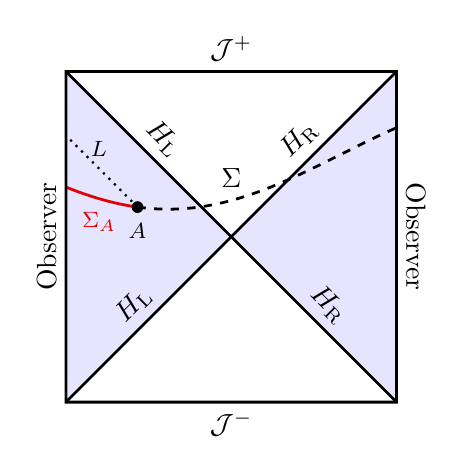
\begin{tikzpicture}[scale=0.7]
	\begin{scope}[transparency group]
		\begin{scope}[blend mode=multiply]
			\path
			+(3,3)  coordinate (IItopright)
			+(-3,3) coordinate (IItopleft)
			+(3,-3) coordinate (IIbotright)
			+(-3,-3) coordinate(IIbotleft)

			;
			\draw(IItopleft) --
			node[midway, above, sloped] {$\mathcal{J}^+$} (IItopright) --
			node[midway, above, sloped] {Observer} (IIbotright)--
			node[midway, below, sloped] {$\mathcal{J}^-$} (IIbotleft) --
			node[midway, above, sloped] {Observer}(IItopleft) -- cycle;

			\fill[fill=blue!10] (-3,3) -- (-3,-3) -- (0,0);

			\fill[fill=blue!10] (3,3) -- (3,-3) -- (0,0);


			\draw[dotted, thick] (-1.7,0.538) -- (-3,1.838);

			\draw[domain=-3:-1.7, smooth, variable=\x, red] plot ({\x}, {sin(deg((\x/2-1)))+1.5});
			\draw[domain=-1.7:3, smooth, variable=\x, black, dashed] plot ({\x}, {sin(deg((\x/2-1)))+1.5});

			\node at (-2.4,0.8) [label = below:\footnotesize{\color{red}$\Sigma_A$}]{};
			\node at (-1.7,0.538) [circle, fill, inner sep=1.5 pt, label = below:\footnotesize{$A$}]{};\node at (-2.4,1.1) [label = above:\footnotesize{$L$}]{};



			\draw  (IItopleft) --  node[midway, above, sloped] {$H_{\rm L}$} (0,0)-- node[midway, above, sloped] {$H_{\rm R}$} (IIbotright)
			(IItopright) --node[midway, above, sloped] {$H_{\rm R}$} (0,0) -- node[midway, above, sloped] {$H_{\rm L}$} (IIbotleft) ;

			\node at (0,1.6) [label=below:$\Sigma$]{};

		\end{scope}
	\end{scope}
\end{tikzpicture}

\end{document}